\documentclass{article}
\usepackage{graphicx,url,paralist}

\begin{document}
\addtolength{\parskip}{0.2cm}
\newcommand{\todoservice}[1]{\vspace{0.2cm} \large \textbf{\underline{TODO Services:}}\\ \normalsize #1 }
\newcommand{\todoapp}[1]{\vspace{0.2cm} \large \textbf{\underline{TODO Application:}}\\ \normalsize #1 }
\title{Documentation to the Online Exercise Assistant}
\author{Sylvia Stuurman}
\date{july 2008}
\maketitle
\begin{figure}[h]
\begin{center}
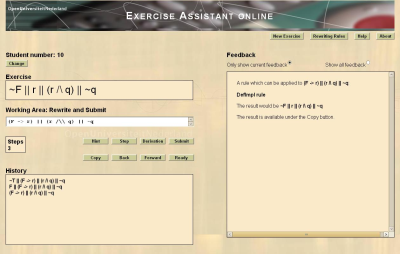
\includegraphics{figures/page-elements.png}
\end{center}
\caption{The Exercise Assistant On-line}\label{figure:screenshot}
\end{figure}
Below, we describe the static and dynamic structure of the code of the Exercise Assistant which uses the strategy-based feedback services.

\section{The HTML and the PHP}
\subsection{The generic part: framework.php}
The generic part of HTML for the Exercise Assistant is bundled in one file, \url{framework.php} which contains several elements which can be questioned and modified dynamically using Javascript, as we will see below. This file is written in PHP, and uses php functions to write the labels in the page for multilanguage usage (we will discuss where and how below). The exact code is shown in appendix~\ref{appendix:framework}. 

\subsubsection{Page elements}
The page elements (see figure~\ref{figure:screenshot}) are:

A \textbf{row of menubuttons} immediately below the header, containing:
	\begin{compactitem}
	\item The \textbf{New Exercise} button, which will invoke a \textbf{generate} function,
	\item The \textbf{Rules}-, \textbf{Help}- and \textbf{About}-buttons, which will cause three different HTML fragment to show,
		\end{compactitem}

A \textbf{left column}, containing:
	\begin{compactitem}
	\item In the OU version, page elements for input and display of the \textbf{student number}.
	\item The \textbf{Exercise Area} where the exercise will be shown (not editable by the user),
	\item The \textbf{Work Area} where the user may rewrite the expression,
	\item The \textbf{Progress Area} which will show how many steps will be needed minimally,
	\item Two \textbf{rows of buttons}:
		\begin{compactitem}
		\item The \textbf{Hint}-button which will invoke the hint function,
		\item The \textbf{Next}-button which will invoke the next function,
		\item The \textbf{Derivation}-button which will invoke the derivation function,
		\item The \textbf{Submit}-button which will invoke the feedback function,
		\item The \textbf{Copy}-button (only visible when there is something to copy) which will invoke the copy function,
		\item The \textbf{Back}-button (only visible when there is something to go back to) which will invoke the back function,
		\item The \textbf{Forward}-button (only visible when there is something to go forward to) which will invoke the forward function,
		\item The \textbf{Ready}-button which will invoke the ready function,
		\item In the domain-specific version, a virtual keyboard
		\end{compactitem}
	\item The \textbf{History Area} which will show the valid steps,
	\end{compactitem}

A \textbf{right column}, containing:
	\begin{compactitem}
	\item two radiobuttons enabling the user to choose between viewing all feedback or (default) only the
	current feedback
	\item a button to clear the feedback area
	\item The \textbf{Feedback Area} whic will show the feedback. There are radio buttons with which the user nmay choose between seeing all feedback, or only the current feedback,
		\end{compactitem}

\subsubsection{Dynamic parts in the Head}
In the head of \url{framework.php} three lines are written dynamically:
\begin{verbatim}
<script type="text/javascript" 
    src="<?php print getLanguage();?>">
</script>
<script type="text/javascript" 
    src="<?php print getLocal();?>">
    </script>
<script type="text/javascript">
    var exercisekind = 
        <?php $kind = getKind(); echo "\"$kind\";"; ?>; 
    var id=421;
</script>\end{verbatim}
We will discuss below where and how these functions are implemented.

\subsubsection{Dynamic labels}
In the body of \url{framework.php}, labels are implemented by php constants, which are given a value in language-dependent php files (see below). An example of such a dynamic label is:
\begin{verbatim}
<input 
    class="menu" 
    type="button" 
    id="aboutButton" 
    value="<?php print About;?>" 
>
\end{verbatim}

\subsection{How to invoke the Exercise Assistant}
At this moment, there are three different ways to use the on-line Exercise Assistant: 
\begin{compactitem}
\item in a \textbf{generic} way, which automatically supports every domain and every exercisekind 
which is supported by the feedback services, 
\item in a way which makes it possible to add \textbf{domain-specific} page elements and page behaviour, 
such as the use of the official symbolss for a domain and a virtual keyboard for input,
\item for OU students, where the student is asked to enter his or her \textbf{studentnumber}.
\end{compactitem}

\subsubsection{Generic}
\textbf{\url{http://ideas.cs.uu.nl/genexas/}} 

This URL shows links to the types of exercises that are
offered by the Strategy-based feedbackservices. The links are hard-coded, but when an
extra service would send a list of types of exercises, this service could be used to 
generate the list of links automatically.

The links on \url{http://ideas.cs.uu.nl/genexas/} have the form of:\\
\textbf{\url{generic.php?exercisekind=Proposition to DNF}}.

The file \url{generic.php} (see appendix~\ref{appendix:generic}):
\begin{compactitem}
\item inludes standard help-, about- and rules files, 
\item includes the file \url{/common/en.php} (see below),
\item defines a function getKind() which returns a string with the chosen exercisekind, and
\item includes the file \url{framework.php} described above (see appendix~\ref{appendix:framework}).
\end{compactitem}

The file \url{en.php}: 
\begin{compactitem}
\item defines the labels to be used for titles and buttons in the page, and
\item implements the function getLanguage() by returning the url of a language-dependent javascript file.
\end{compactitem}

The structure of these files is as follows:

\textbf{\url{/genexas/}} \\
 \url{index.php} (see appendix~\ref{appendix:index})\\
 \url{generic.php} (see appendix~\ref{appendix:generic})

\textbf{\url{/genexas/common/}}\\
 \url{en.php} (conmstants for labels, as: define("About", "About");)\\
 \url{framework.php} (see appendix~~\ref{appendix:framework}) 

\textbf{\url{/genexas/common/en}}\\
 \url{about.php} (a default about-text)
 \url{help.php} (a default help-text)
 \url{rules.php} (a default text about rewriting rules)
	
\todoservice{Create a service which returns a list of exercisekinds}

\todoapp{Use that service to create \url{http://ideas.cs.uu.nl/genexas/} dynamically}
	
\textbf{Language}

The default language is English, but using the language options of the Apache server, it would be easy to switch to multilanguage. In that case, instead of a single \url{index.php}, there would be an \url{index.en.php} and an \url{index.nl.php} (etc), and instead of including the file with English names, the appropriate language file would be included.

The structure would become as follows:

\textbf{ \url{/genexas/}} \\
 \url{index.php} (see appendix~\ref{appendix:index})\\
 \url{generic.en.php} (to invoke the English version)\\
 \url{generic.nl.php} (to invoke the Dutch version)\\
 More languages can be added\\

\textbf{\url{/genexas/common/}}\\
 \url{en.php} (labels defined: define("About", "About");)\\
 \url{nl.php} (labels defined: define("About", "Over");)\\
 More languages can be added\\
 \url{framework.php} (see appendix~~\ref{appendix:framework}) 

\textbf{\url{/genexas/common/en}}\\
 \url{about.php} (a default about-text)\\
 \url{help.php} (a default help-text)\\
 \url{rules.php} (a default text about rewriting rules)
 
 \textbf{\url{/genexas/common/nl}}\\
 \url{about.php} (a default about-text)\\
 \url{help.php} (a default help-text)\\
 \url{rules.php} (a default text about rewriting rules)\\
 More language subdirectories can be added
 
 \todoapp{Complete the lenguage-dependent files for the Dutch language}

\subsubsection{Domain-specific}
\textbf{\url{http://ideas.cs.uu.nl/genexas/logic/todnf/index.en}}

Another way to use the Exercise Assistant is through URL's pointing to domain-specific Exercise Assistants. At this moment, there are two such URL's: 

\textbf{\url{http://ideas.cs.uu.nl/genexas/logic/todnf/index.php}} \\ (which makes use of the multilanguage facility; because only English is fully implemented, it is safest to use \url{http://ideas.cs.uu.nl/genexas/logic/todnf/index.en}) 

\textbf{\url{http://ideas.cs.uu.nl/genexas/math/relationalgebra/index.php}} \\ (for which the same applies, so preferrably use \url{http://ideas.cs.uu.nl/genexas/math/relationalgebra/index.en)}.

The difference with the so-called generic url is, that it is possible to integrate domain-specific HTML and Javascript, for instance to enhance the user interface by providing real mathematical symbols instead of ASCII characters for input and output.

The language-specific \url{index.en.php} (see appendix~\ref{appendix:todnf:en}):
\begin{compactitem}
\item inludes  help-, about- and rules files, (here, either the defaults may be used or domain-specific texts),
\item includes the file \url{/genexas/common/en.php} (see above), and 
\item includes the file \url{index.php}.
\end{compactitem}

This file, \url{index.php} (see appendix~\ref{appendix:todnf}):
\begin{compactitem}
\item implements getLocal() to produce code for using domain-specific symbols, 
\item implements getKind() to return the correct exercisekind string, and
\item includes \url{framework.php} (see appendix~\ref{appendix:framework}).
\end{compactitem}

\subsubsection{OU specific}
\textbf{\url{http://ideas.cs.uu.nl/genexas/logic/todnf/ou/}}

The third possibility to use the Exercise Assistant is for OU students, asking them for their student number.

The file \url{/genexas/logic/todnf/index.php}:
\begin{compactitem}
\item inludes  help-, about- and rules files, (here, either the defaults may be used or domain-specific texts),
\item implements getKind() to return the appropriate exercisekind string,
\item implements getLocal() to return the file \url{communication.js}, specifically for the student number (seel below),
\item includes the file \url{/genexas/common/en.php} (see above) and 
\item includes the file \url{framework.php} described above (see appendix~\ref{appendix:framework}).
\end{compactitem}

\section{Javascript}
The behaviour of the Exercise Assistant is implemented in Javascript. We will describe the different files here.

\subsection{/genexas/common/javascript/services.js}
This file contains functions to call the strategy-services. Each function requires the input which is needed to call the service, and a callback function. The services are called through an asynchronous Ajax call, and the callback function will be called when the result has arrived.

The functions are:
\begin{compactitem}
\item function ss\_generate(number, callback) (code: see appendix~\ref{appendix:services}),
\item function ss\_getReady(state, callback),
\item function ss\_getHint(location, state, callback),
\item function ss\_getNext(state, callback),
\item function ss\_getDerivation(state, callback,
\item function ss\_getRemaining(state, callback) ,
\item function ss\_getFeedback(state, newexpression, callback).
\end{compactitem}

The data type of number is an integer.

The data type of state is defined as follows:
\begin{verbatim}
function State(id, prefix, exercise, simpleContext) {
    this.id = id;
    this.prefix = prefix;
    this.exercise = exercise;
    this.simpleContext = simpleContext;
}
\end{verbatim}
Here, id will be produced by the application itself, to discern between responses of services that might arrive in a non-chronological order. In addition, the student number could be used to produce id's. The other three elements of State are strings, received through the services.

%Location also comes as a string, and is received through the services.

\subsection{/genexas/common/javascript/communication.js}
This file is a mediator between the elements of the HTML page and the \url{services.js}-functions. 

For each action that the user interface allows to, there are a pair of functions: one that knows where to get the appropriate paramteres from, and one that knows how to display the results. The display function is used as the callback function when calling a function from \url{services}.js.

An example of the code is shown in appendix~\ref{appendix:communication}). The code is relatively easy to read, when you realise that:
\begin{verbatim}
$('exercise')
\end{verbatim}
is a function returning the page element with the id `exercise'.

\subsection{/genexas/common/javascript/help.js}
Apart from some utility functions, this file provides the code for the history within the application, which makes it possible for the user to go back and forth.

The two concepts which are used to implement the history are the \url{snapshot} and the \url{historykeeper}:
\begin{verbatim}
/**
 * a snapshot contains:
 * - exercise. Is the exercise that is to be solved, 
 *   and will stay the same until a new exercise is generated
 * - feedback: Is the content of the feedback area
 * - history: Is the content of the History area
 * - work: is the content of the work area; 
 *   this is a combination of a state and a location
 * - state, which contains: 
 *     the id of the exercise, 
 *     the prefix, 
 *     the current *valid* expression, 
 *     and the simpleContext
 * - copy: is a copy of the last valid state; 
 * - location
 * - steps
 * 
 * snapshot is the current snapshot
 * it is a Hash object, so we can add new key-value pairs if necessary
 */
var snapshot;
/**
 * Our historykeeper will be an array filled with hashObjects, 
 * containing the variable contents of the page elements
 * statePointer points out the index of the snapshot within the historyList
 */
var historyKeeper = new Object();
historyKeeper.historyList = new Array();
historyKeeper.statePointer = -1;
\end{verbatim}

The historyKeeper has the following functions:
\begin{itemize}
\item addSnapshot(snapshot)
\item newSnapshot()
\item update(state) (a new snapshot is taken, with only the state different from the previous one)
\item addFeedback() (a new snapshoy is taken, with only the contents of the feedbackfield different from the previous one)
\item addCopy(state) (a state is kept to copy from)
\item removeCopy() (there is no extra state to remember)
\end{itemize}

The functions goBack and goForward make use of the historyKeeper.

\subsection{/genexas/logic/todnf/ou/communication.js}
The file \url{framework.php} contains page elements that show an input field for the student number, a field to display it, and a button with which the student may tell the number is wrong. The style sheet for the application (\url{/genezas/css/exas.css}) hides those elements by default.

This file dynamically makes the appropriate elements visible. It tries to store the number in a cookie (whioch will mean that the student doesn't have to enter the number each time), but there is no prolem when the user has turned off that possibility.

At this moment, the student number is used as the id in the calls to the feedback service. However, we should change that.

\todoapp{Generate a unique id for each serice call, to discriminate between two responses} 

\todoapp{Use the student number to create an id from which the student number can be extracted at the Haskell-side}

\todoapp{Use the student number to send the data of each service call to a url which logs those data per student number}


\appendix
\section{HTML code for the Exercise Assistant}
\subsection{/genexas/common/framework.php}\label{appendix:framework}
\subsubsection{The HEAD}
\begin{verbatim}
<!DOCTYPE HTML PUBLIC "-//W3C//DTD HTML 4.01//EN"
    "http://www.w3.org/TR/html4/strict.dtd">
<html>
<head>
<meta http-equiv="Content-Type" 
    content="text/html;charset=utf-8" >

<title>OU Exercise Assistant On-line</title>
<link rel="stylesheet" type="text/css" 
    href="/genexas/css/exas.css" >
<link rel="shortcut icon" type="image/x-icon" 
    href="/genexas/css/favicon.ico" >
<script type="text/javascript" 
    src="/genexas/common/javascript/prototype-1.6.0.2.js">
    </script> 
<script type="text/javascript" 
    src="/genexas/common/javascript/help.js">
    </script>
<script type="text/javascript" 
    src="/genexas/common/javascript/services.js">
    </script>
<script type="text/javascript" 
    src="/genexas/common/javascript/communication.js">
    </script>
<script type="text/javascript" 
    src="<?php print getLanguage();?>">
</script>
<script type="text/javascript" 
    src="<?php print getLocal();?>">
    </script>
<script type="text/javascript">
    var exercisekind = 
        <?php $kind = getKind(); echo "\"$kind\";"; ?>; 
    var id=421;
</script>
<script type="text/javascript" 
    src="/genexas/common/javascript/init.js">
    </script>
</head>
\end{verbatim}
\subsubsection{The BODY}
\textbf{The header and menubuttons}
\begin{verbatim}
<h1>Exercise Assistant online</h1>
<div id="exasdiv">
<input class="menu" type="button" 
    id="aboutButton" value="<?php print About;?>" >
<input class="menu" type="button" 
    id="helpButton" value="<?php print Help;?>" >
<input class="menu" type="button" 
    id="rulesButton" value="<?php print Rules;?>" >
<input class="menu" type="button" 
    id="generateButton" value="<?php print NewExercise;?>" >
<br class="clear" >
\end{verbatim}
\textbf{The left column}
\begin{verbatim}
<div class="column left">

  <div id="numberinput" style="display: none">
    <h3>Please first fill in your student number</h3>
    <textarea id="number" rows="1" cols="12"></textarea>
    <input type="button" id="numberbutton" value="Enter">
  </div><!-- end div numberinput -->
	
  <div id="numberdisplay"  style="display: none">
    <h3 id="studentnumber"></h3>
    <input type="button" id="changenumberbutton" 
    value="Change">
  </div><!-- end div numberdisplay -->
	
  <h3><?php print Exercise;?></h3>
  <div id="exercise" >
  </div><!-- end div exercise -->

  <h3><?php print WorkArea;?></h3>

	<textarea id="work" rows="2" cols="40" >	
	</textarea><!-- end work area -->
	
  <!-- the buttons -->
  <input class="minibutton" 
    id="submitbutton" type="button" 
    value="<?php print Submit;?>" >	
  <input class="minibutton" 
    id="derivationbutton"  type="button" 
    value="<?php print Derivation;?>" >
  <input class="minibutton" 
    id="nextbutton"  type="button" 
    value="<?php print Step;?>" >
  <input class="minibutton" 
    id="hintbutton" type="button" 
    value="<?php print Hint;?>" >
  <div id="progress">Steps<br>0
  </div><!-- end div progress -->
	
  <br class="clear">
  <input class="minibutton" type="button" 
    id="readybutton" value="<?php print Ready;?>" >
  <input class="minibutton" type="button" 
    id="forwardbutton" value="<?php print Forward;?>" >
  <input class="minibutton" type="button" 
    id="undobutton" value="<?php print Back;?>" >
  <input class="minibutton" type="button" 
    id="copybutton" value="<?php print Copy;?>" >
  <!-- end buttons -->
  <br>
	
  <h3><?php print History;?></h3>
  <div id="history">
  </div><!-- end div history -->

</div><!-- end div column left -->
\end{verbatim}
\textbf{The right column}
\begin{verbatim}
<div class="column right">

  <h3><?php print Feedback ?></h3>
  <label class="feedbacklabel"><?php print ChooseClear;?>
    <input type="radio" name="feedbackchoice" 
      id="feedbackclearchoice" 
      checked value="chooseclear" >
  </label>
  <label class="feedbacklabel"><?php print ChooseKeep;?>
    <input type="radio" name="feedbackchoice"  
      id="feedbackeepchoice" 
      value="choosekeep" >
  </label>
  <input type="button" 
    id="clearbutton" 
    value="<?php print Clear;?>"  style="display: none">
		
  <div id="feedback" class="clear"><?php print Welcome;?>
  </div><!-- end div feedback -->

</div><!-- end div column right -->
\end{verbatim}
\textbf{The Help areas}
\begin{verbatim}
<div id="rules" class="helparea invisible">
  <input class="helpbutton" 
    id="closerulesButton" type="button" 
    value="<?php print Close;?>" >
    <?php rules();?>
</div><!-- end div rules -->

<div id="help" class="helparea invisible">
  <input class="helpbutton"  
    id="closehelpButton" type="button" 
    value="<?php print Close;?>" >
    <?php help();?>
</div><!-- end div help -->

<div id="about" class="helparea invisible">
  <input class="helpbutton"  
    id="closeaboutButton" type="button" 
    value="<?php print Close;?>" >
    <?php about();?>
</div><!-- end div about -->

</div><!-- end div exas -->
</body>
</html>
\end{verbatim}
\subsection{/genexas/generic.php}\label{appendix:generic}
\begin{verbatim}
<?php
function rules() {
    include_once("common/en/rules.html");
}
function help() {
    include_once("common/en/help.html");
}
function about() {
    include_once("common/en/about.html");
}
function getKind() {
    return $_GET["exercisekind"];
}
function getLocal() {
    return "";
}
include_once("common/en.php");
include("common/framework.php");
?>
\end{verbatim}
\subsection{/genexas/index.php}\label{appendix:index}
\begin{verbatim}
<!DOCTYPE HTML PUBLIC "-//W3C//DTD HTML 4.01//EN"
    "http://www.w3.org/TR/html4/strict.dtd">
<html>
<head>
<meta http-equiv="Content-Type" 
    content="text/html;charset=utf-8" >

<title>OU Exercise Assistant On-line</title>
<link rel="stylesheet" 
    type="text/css" 
    href="/genexas/css/exas.css" >
<link rel="shortcut icon" 
    type="image/x-icon"
    href="/genexas/css/favicon.ico"  >
</head>

<h1>Exercise Assistant online</h1>
<p><a href="generic.php?exercisekind=Proposition%20to%20DNF">
    Proposition Logic</a></p>
<p><a href="generic.php?exercisekind=To%20conjunctive%20normal%20form">
    Relational Algebra</a></p>
</body>
</html>
\end{verbatim}
\subsection{/genexas/proplogic/todnf/index.en.php}\label{appendix:todnf:en}
\begin{verbatim}
<?php
function rules() {
  if (file_exists("./en/rules.html")) {
    include_once("./en/rules.html");
  }
  else {
    if (file_exists("./../en/rules.html")) {
      include_once("./../en/rules.html");
    }
    else {
      include_once("../../common/en/rules.html");
    }
  }
}
function help() {
  if (file_exists("./en/help.html")) {
    include_once("./en/help.html");
  }
  else {
    if (file_exists("./../en/help.html")) {
      include_once("./../en/help.html");
    }
    else {
      include_once("../../common/en/help.html");
    }
  }
}
function about() {
  if (file_exists("./en/about.html")) {
    include_once("./en/about.html");
  }
  else {
    include_once("../../common/en/about.html");
  }
}
include_once("../../common/en.php");
include_once("index.php");
?>
\end{verbatim}
\subsection{/genexas/proplogic/todnf/index.php}\label{appendix:todnf}
\begin{verbatim}
<?php
// if there is a special user interface for the domain
function toetsen() {
  if (file_exists("../keys.php")) {
    include_once("../keys.php");
  }
}
function getKind() {
  return "To%20conjunctive%20normal%20form";
}
include_once("../../common/framework.php");
?>
\end{verbatim}
\section{Javascript code for the Exercise Assistant}
\subsection{/genexas/common/javascript/services.js}\label{appendix:services}
One example of the code.
\begin{verbatim}
// The url for the services
var url = "/cgi-bin/service.cgi";
/**
 *  Generation of a new exercise. 
 * Input: an integer
 * Output: a state object 
 * The output is passed to the callback function
 */
function ss_generate(number, callback) {
  var myAjax = new Ajax.Request(url, {   
    parameters : 
      'input={ 
        "method" :"generate", 
        "params" : ["'+ exercisekind + '", ' + number + '], 
        "id" : ' + id + '}',	 
      onSuccess : function(response) {	
        var resJSON = parseJSON(response.responseText);
        var error = resJSON.error;
        if (error == null) {
          result = resJSON.result;
          var state = new State(result[0], result[1], result[2], result[3]);
          callback(state);
        }
        else {
          alert(wrong);
        }			
      },
      onFailure: function() { 
        alert(wrong); 
      } 
  });
}
\end{verbatim}
\subsection{/genexas/common/javascript/communication.js}\label{appendix:communication}
One example of the code to handle call a service and handle the result.
\begin{verbatim}
/**
 * Generate a new exercise,
 * A function to call the service and a display function
 */
function generate() {
  ss_generate(5, displayExercise);
}
/**
 * Display new exercise.
 * Updates the exercise area, the work area and the history area.
 * A new snapshot is taken for the back button
 */
function displayExercise(state) {
  closeallhelp();
	
  setInvisible($('copybutton'));
  var task = state.exercise;
  $('exercise').update(task);
  $('work').value = task;
  $('history').update(task);
  ss_getRemaining(state, function(number) {
    $('progress').update('Steps<br> ' + number); 
    historyKeeper.newSnapshot(state);
  } );
  adjustHeight($('exercise'), task, 40, 40);
  adjustRows($('work'), task, 40);
}
\end{verbatim}
\end{document}